\newpage
\section{Implementation}

The exchange of messages between server-client and server-server must be done in a secure way. This means that all messages must be confidential, thus they can only be read by the entities which are supposed to read them.

\subsection{Security mechanisms implementation}

\begin{itemize}
    \item First of all, the Client and the Server must exchange a shared key using the \textbf{Diffie-Hellman} method. This shared key will be used to encrypt the plaintext to be sent, in a symmetric key encryption scheme. 
    \item Next, the Client and the Server must exchange their signed public key certificates (see Figure \ref{fig:pubkeyexchange})
    \item To exchange the messages in a secure way, we will use an hybrid cipher (simultaneous use of symmetric cipher and asymmetric cipher). The algorithm to be used by the asymmetric cipher will be RSA, and the algorithm for the symmetric cipher will be AES.
    \item The client will be identified in the system by one’s “id”. This will be obtained from the digest of the user’s public key certificate, extracted from one’s Citizen Card. So, the “id” is going to be used to identify the user in a unique way.
    \item The must be a control of integrity on the messages exchanged (non corrupted data). 
    
    We will use an Encrypt-then-MAC architecture, in which the MAC is computed from the cryptogram. 
    
    After the hash function (HMAC with SHA256), the digest (result) will be encrypted by the user’s private key (the one from the Citizen Card) and so we can guaranty the authentication and integrity control of all messages - signature. In other words, using this MAC we can confirm that the message received by a client came from the stated sender (authenticity) and has not been changed in the process.
\end{itemize}

\begin{figure}[H]
\center
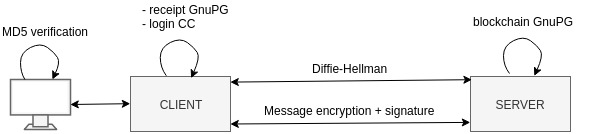
\includegraphics[height=3cm]{sections/img/client-server.jpg}
\caption{Client-Server interaction diagram.}
\label{fig:clientserversecurity}
\end{figure}

\begin{figure}[H]
\center
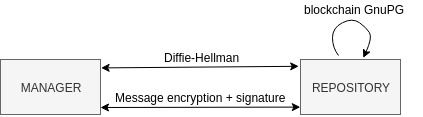
\includegraphics[height=2.7cm]{sections/img/server-server.jpg}
\caption{Server-Server interaction diagram.}
\label{fig:serverserversecurity}
\end{figure}

\vspace*{5mm}

\subsubsection{Certificate Validation and Public Key exchange}
On the first connection between the server and the client(which can be a server), the information exchanged is sent in plaintext between both entities. This happens because no participant knows the other.
In this case the first thing to do is getting information on the other participant. Normally to do this, the agents will need to exchange certificates (or public keys generated from the certificates).

The exchange of the certificates between the two servers and between the client and the server is processed as follows (considering Server A as a Client and Server B as a Server) (see Figure \ref{fig:pubkeyexchange}):
\begin{enumerate}[font=\bfseries]
    \item First, the servers must have a private key, from which they will generate a certificate. This certificate will generate a valid public key from the server which generated it.
    \item The Server (might be the repository or the manager) sends its own self-signed certificate to the other Server or Client.
    \item The Client will then validate the certificate chain. If it is invalid, the certificate is discarded. If it is valid, the Client will send a signed challenge encrypted with the Server's public key and its own certificate attached.
    \item The Server will also validate the Client's certificate chain and if it is valid, it will reply to the challenge with a signed answer to it, which must be send encrypted with the Client's public key.
\end{enumerate}
On the first connection from all parties the connection is insecure, so as the fist connection is started, we don't expect that someone will try to act as a server, and provide their certificates as a normal attacker would do.

\begin{figure}[H]
\center
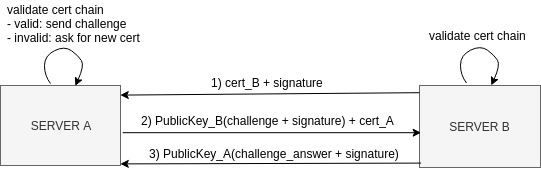
\includegraphics[height=4cm]{sections/img/certs.jpg}
\caption{Public Key certificates exchange diagram.}
\label{fig:pubkeyexchange}
\end{figure}
\vspace*{5mm}

Upon exchanging certificates, the servers can get the public key of the other participant. This means that from now on, the communication can be done using the public keys stored in the known certificates.

\vspace*{5mm}

\subsection{Message  Security}
Upon knowing that the messages should be exchanged without compromising the  information, we are forced to treat the channels where those message are being sent as insecure.
The simplest way to share the messages on a insecure channel is to send so that only each entity can read them.
We will now explain the way our system will encrypt and decrypt the messages.
\subsubsection{Message encryption}\label{sssec:num411}

The encryption of the exchanged messages, will be processed the same way for the client-server communications and the server-server communications (manager server and repository server). Next, we will list the flow for processing the encryption.                   
In this flow (see Figure \ref{fig:messageencrypt}), the generic \textbf{client}, who wants to send a message to the \textbf{server}, can also be a server (since there are two of them which have a different purpose).
 
\begin{enumerate}[font=\bfseries]
    \item The Client obtains the public key of the Server on the first connection;
    \item The message is encrypted with a Diffie-Hellman symmetric key (AES) calculated for the current session;
    \item Process the symmetric key with a hash function (SHA256), so it can be later used in the HMAC function;
    \item The Client encrypts the original symmetric key using Server’s public key (RSA);
    \item The encrypted symmetric key is joined (see .5) with the encrypted message (see .3) and processed in a hash function (HMAC SHA256, using the key of .4);
    \item Encrypt the result of the hash (digest) with the private key of Client.
\end{enumerate}

The sent message will look like as follows:

\begin{equation}\label{eq:1}
\begin{split}
    message=encrypted\_message + encrypted\_symmetricKey +encrypt\_PK(\\
    hmacsha256(hashed\_key,(encrypted\_message +encrypted\_symmetricKey))\\
    )
\end{split}
\end{equation}

The message(\ref{eq:1}) will be sent in a JSON format, where each field is well defined in order to make the decryption process easier.

\vspace*{5mm}

\begin{figure}[H]
\center
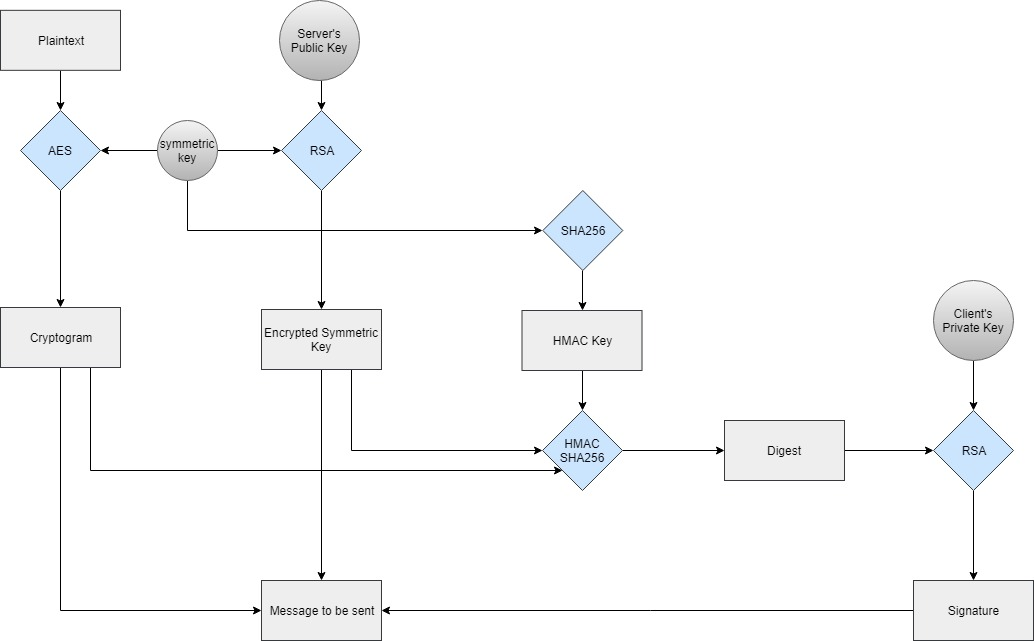
\includegraphics[height=10cm]{sections/img/encryption.jpg}
\caption{Message encryption diagram.}
\label{fig:messageencrypt}
\end{figure}

\vspace*{5mm}

\subsubsection{Message decryption}
To revert the \textbf{encryption} made before, and read  the contents the message, the \textbf{Server} will need to follow a decryption flow:

\begin{enumerate}[font=\bfseries]
    \item Obtain Client's public key;
    \item Decrypt the received HMAC with said key;
    \item Use his private key to decrypt the symmetric key received;
    \item Compute the Hash (SHA256) of the symmetric key;
    \item Compute the HMAC (SHA256) with the received encrypted message and encrypted symmetric key, using the result of the hash of the decrypted symetric key (.4) as the HMAC function key;
    \item Compare both HMAC’s (.5 with .2’s result) and,
    \item If the HMAC’s match (authenticity confirmed), use the symmetric key to decrypt the message (data) received.
\end{enumerate}

\begin{figure}[H]
\center
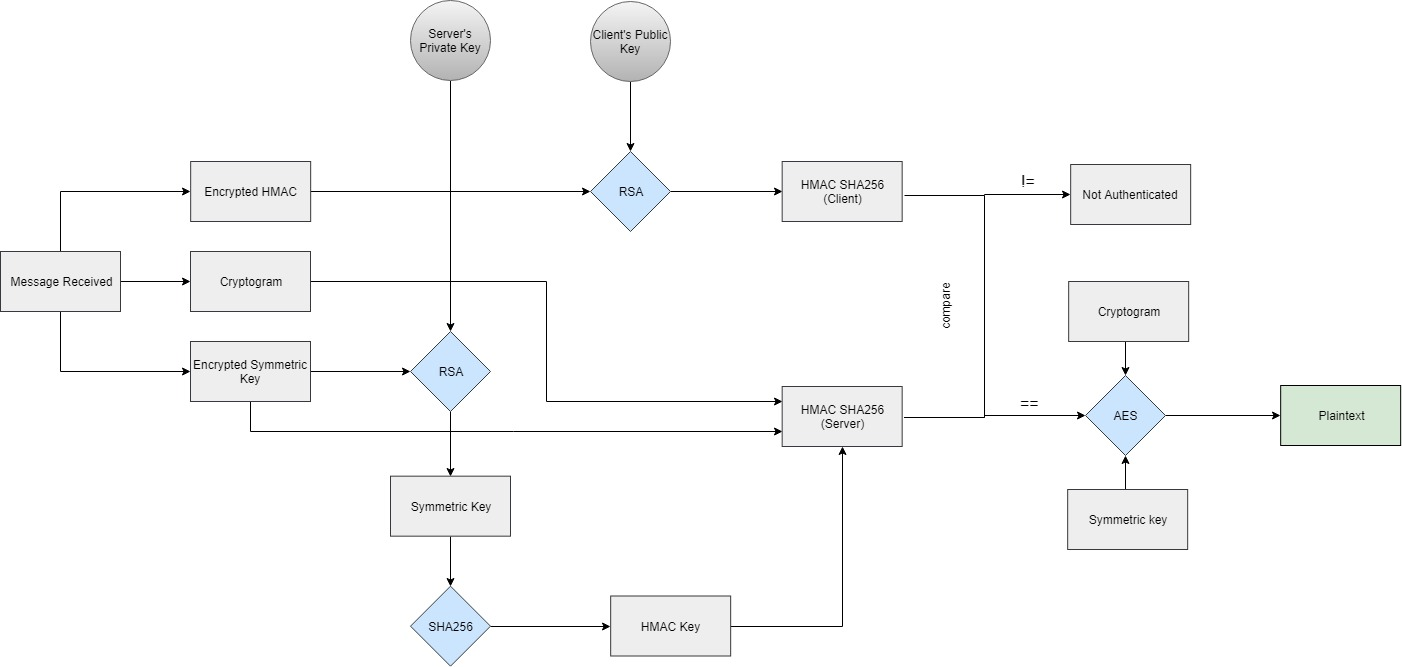
\includegraphics[height=8cm]{sections/img/decryption.jpg}
\caption{Message decryption diagram.}
\label{fig:messagedecrypt}
\end{figure}

\vspace*{5mm}

\subsection{Storage Security}
As we have seen before, all information exchanged will be secure while the memory is volatile. But we also need to secure it in the non-volatile memory. The best alternative, we have encountered is the use of the GNUPG (see Figure \ref{fig:serverserversecurity}) for encrypting all the files with a master password for each server:
\begin{itemize}
    \item On the Client's side (user), there will be receipts stored in files and in the Repository Server there will be a file containing the auction's data. Both files will be encrypted using GnuPG (GNU Privacy Guard).
    \item The user will calculate the MD5 of each receipt stored (see Figure \ref{fig:clientserversecurity}). Every time one wants to use a receipt, one will calculate the MD5 of the current receipt and compare it to the pre-calculated MD5. If they do not match, the receipt might have been adulterated.
    \item The user will be authenticated by the system through a log in on the system's client interface. He/She must insert the Cartão de Cidadão in a card reader and everytime there is the need to sign messages the user must insert their PIN in order for the private key to be used.
\end{itemize}



